\documentclass[]{article}
\usepackage{amsmath}
\usepackage{amssymb}
\usepackage{verbatim} %con verbatim escribes bloques de texto con letra mono.
\usepackage{graphicx} %para insertar imagenes, cuando meta yo una usa el codigo de ejemplo
\usepackage{listings}
\usepackage{fullpage}
\usepackage{color}
\usepackage{fancyvrb}
\usepackage[spanish]{babel}
\usepackage[utf8]{inputenc} %Para usar acentos directamente en latex
\usepackage{hyperref} %Para que el indice tenga hiperenlaces y si quieres poner los tuyos
\hypersetup{%
	pdfborder = {0 0 0}
}

\definecolor{mygreen}{rgb}{0,0.6,0}
\definecolor{mygray}{rgb}{0.5,0.5,0.5}
\definecolor{mymauve}{rgb}{0.58,0,0.82}

%Para insertar código: crea un recuadro con texto mono y lineas enumeradas. Puedes referenciar un fichero y no copiar y pegar aquí.
\lstset{ %
	backgroundcolor=\color{white},   % chohttp://xdxd.com/ose the background color; you must add \usepackage{color} or \usepackage{xcolor}
	basicstyle=\footnotesize,        % the size of the fonts that are used for the code
	breakatwhitespace=false,         % sets if automatic breaks should only happen at whitespace
	breaklines=true,                 % sets automatic line breaking
	captionpos=b,                    % sets the caption-position to bottom
	commentstyle=\color{mygreen},    % comment style
	frame=single,                    % adds a frame around the code
	keepspaces=true,                 % keeps spaces in text, useful for keeping indentation of code (possibly needs columns=flexible)
	numbers=left,                    % where to put the line-numbers; possible values are (none, left, right)
	numbersep=5pt,                   % how far the line-numbers are from the code
	numberstyle=\tiny\color{mygray}, % the style that is used for the line-numbers
	rulecolor=\color{black},         % if not set, the frame-color may be changed on line-breaks within not-black text (e.g. comments (green here))
	showspaces=false,                % show spaces everywhere adding particular underscores; it overrides 'showstringspaces'
	showstringspaces=false,          % underline spaces within strings only
	showtabs=false,                  % show tabs within strings adding particular underscores
	stepnumber=1,                    % the step between two line-numbers. If it's 1, each line will be numbered
	stringstyle=\color{mymauve},     % string literal style
	tabsize=4,
	inputencoding=utf8,
	title=\lstname                   % show the filename of files included with \lstinputlisting; also try caption instead of title
}



\title{Seguridad}
\author{José Luis Cánovas Sánchez - 48636907A\\Ezequiel Santamaría Navarro - 20096517Z}

\begin{document}

\maketitle

\begin{abstract}
En esta memoria se describe el desarrollo del apartado 2.1 de las prácticas de Seguridad: Despliegue de servicios de gestión de identidad avanzados mediante biometría y tecnologías SAML y OAuth.
\end{abstract}

\tableofcontents


\section{Introducción}

Como grupo 3 de prácticas, desplegaremos las organizaciones 31 y 32.
El trabajo en grupo ha consistido en que ambos hemos desarrollado y configurado todo conjuntamente, lo que se refleja en nuestro repositorio git de GitHub, donde subimos los scripts de instalación con los que automatizamos la práctica, pues preferimos no usar máquinas virtuales, por los problemas de fluidez y tamaño de las máquinas virtuales. Así podemos trabajar con unos pocos megas de scripts y capturas en cualquier ordenador.


%\begin{center}
%	\includegraphics[width=1\linewidth]{images/}
%\end{center}


\section{Autenticación biométrica}

Desarrollamos una aplicación para \textbf{comparación}, \textbf{identificación} y \textbf{verificación} de huellas dactilares.

\subsection{Funcionamiento de la aplicación}

Primero vamos a ver \textbf{cómo funciona} la aplicación desarrollada, y una vez conocemos todas las funcionalidades que ofrece, veremos cómo lo hemos implementado.

\hfil

Cuando abrimos la aplicación nos encontramos con 4 paneles, dos superiores donde se mostrarán las imágenes de las huellas dactilares, dos inferiores, el izquierdo con los botones de las funcionalidades del programa, además del menú superior, y un panel que muestra en texto la descripción de los resultados mostrados.

Los dos primeros botones, \textit{Calcular 1 huella} y \textit{Comparar 2 huellas} no dependen de la base de usuarios del programa.

Al pulsar el primero se abre un explorador de ficheros para abrir la foto de una huella dactilar. El programa entonces muestra la imagen seleccionada a la izquierda y la analizada a la derecha (se indica así en el cuarto panel), y su matriz en el cuadro de texto correspondiente del tercer panel.

El botón de \textit{Comparar 2 huellas} abre dos veces el explorador de ficheros, y muestra las imágenes analizadas, sus matrices y el porcentaje de similitud entre las huellas.


\begin{center}
	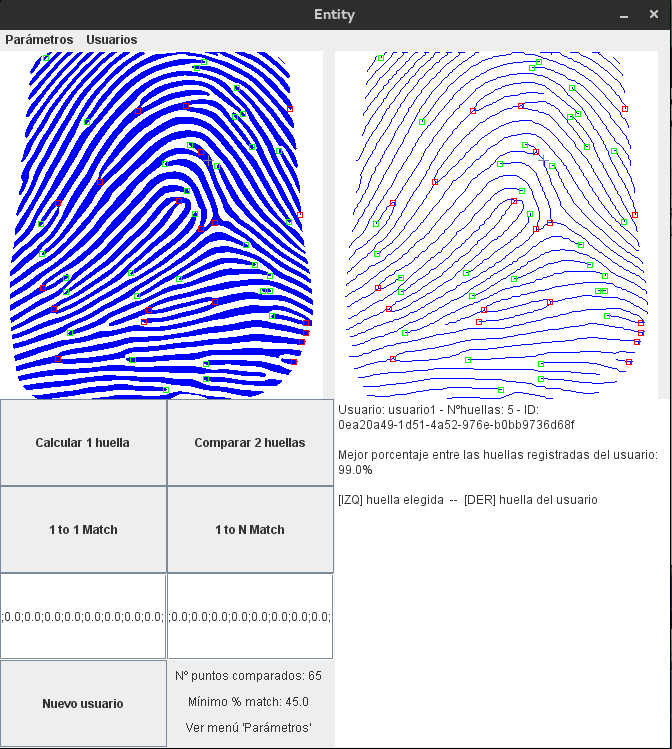
\includegraphics[width=0.55\linewidth]{images/huellas/5.png}

	\textit{Ventana de la aplicación}
\end{center}

Los siguientes botones sí usan la funcionalidad de usuarios del programa. Cuando pulsamos \textit{Nuevo usuario} se abre una ventana nueva donde introducimos su nombre y seleccionamos tantas huellas como queramos para dicho usuario.

\begin{center}
	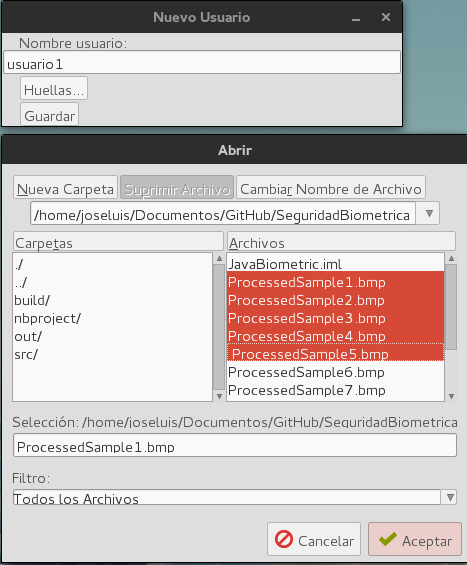
\includegraphics[width=0.45\linewidth]{images/huellas/1.png}

	\textit{Ventana para registrar un nuevo usuario}
\end{center}


Al pulsar en \textit{1 to 1 Match} se realiza una \textbf{verificación} entre un fichero que selecciones en el explorador de ficheros y un usuario de entre los registrados, que se puede elegir de una lista desplegable en una nueva ventana.

\begin{center}
	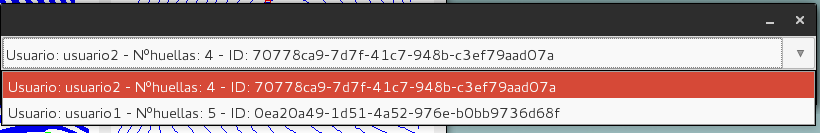
\includegraphics[width=1\linewidth]{images/huellas/3.png}

	\textit{Listado de usuarios para la verificación}
\end{center}

Al pulsar en \textit{1 to N Match} se realiza la comparación de un nuevo fichero que se elija, y todos los usuarios registrados, mostrando la información de los usuarios con las huellas que superan el porcentaje de coincidencia. Se puede probar bajando a un 10\% dicho porcentaje, se mostrará una lista donde cada usuario aparece una sola vez, si alguna de sus huellas supera el porcentaje, y se indica el porcentaje de coincidencia de su huella más coincidente.

\begin{center}
	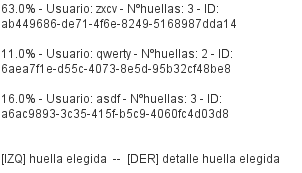
\includegraphics[width=0.5\linewidth]{images/huellas/2.png}

	\textit{Listado de usuarios con huellas que superan el matching}
\end{center}


Por último tenemos las opciones de configuración del menú superior. Tenemos un menú de \textit{Usuarios} con las mismas opciones que ya hemos visto, y un menú de \textit{Parámetros} donde podemos modificar el número de puntos que usará el programa para comparar dos huellas dadas, y el porcentaje mínimo de similitud entre dos huellas para considerar que son de la misma persona.

\begin{center}
	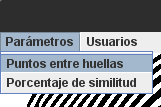
\includegraphics[width=0.25\linewidth]{images/huellas/4.png}

	\textit{Menú Parámetros}
\end{center}

\begin{center}
	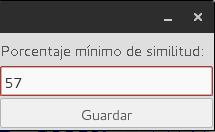
\includegraphics[width=0.25\linewidth]{images/huellas/6.png}

	\textit{Ventana emergente para configurar el porcentaje de similitud}
\end{center}

\begin{center}
	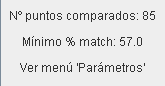
\includegraphics[width=0.25\linewidth]{images/huellas/7.png}

	\textit{Cuadro de texto en el tercer panel con la información de los parámetros actuales}
\end{center}



\subsection{Implementación}


Ahora veamos cómo lo hemos \textbf{implementado}.
\hfill

En la carpeta \textit{src} del proyecto encontramos el fichero \textit{CatalogoUsuarios.java}, donde por un \textit{HashMap} guardamos los usuarios registrados, haciendo uso de la clase \textit{Usuario}, y ofreciendo métodos para la \textbf{identificación}, método \textit{findMatch()}, que devuelve el conjunto de los usuarios que superan el porcentaje de similitud, como se ha descrito en el apartado de la interfaz de usuario.

El fichero \textit{Usuario.java} implementa la representación de cada usuario registrado, mediante un identificador único (asignado automáticamente), un nombre y un conjunto de huellas, representadas por la clase \textit{Huella}. La clase ofrece dos métodos para la \textbf{verificación}, uno que devuelve su huella que mejor coincidencia tiene con otra huella pasada como parámetro, y el otro método devuelve el \textit{double} con el porcentaje de coincidencia.

El fichero \textit{Huella.java} guarda la representación de las huellas dactilares, creándolas a partir del fichero pasado, ofreciendo los métodos para recuperar las imágenes, matriz de la huella calculada (como matriz o string) y el método \textit{coincidencia()} que devuelve el \textbf{porcentaje} de coincidencia entre la huella y otra pasada por parámetro, usando tantos \textbf{puntos} para comparar como configure el usuario.

\hfill

Con estos tres ficheros y la biblioteca \textit{BiometrikSDK} tenemos lo necesario para manipular las huellas y usuarios.

\hfill

En el fichero \textit{ProgramVariables.java} tenemos como parámetros globales los valores que puede ajustar el usuario, número de puntos de comparación entre huellas, y porcentaje mínimo de éxito.

En el fichero \textit{NuevoUsuarioForm.java} se implementa la ventana de registro de un nuevo usuario, y en la acción del botón \textit{Guardar...} se crea el nuevo objeto \textit{Usuario} y se guarda en el catálogo de usuarios.

En el fichero \textit{CEntityForm.java} se implementa el resto de la funcionalidad, la ventana principal del programa, junto a los métodos de los botones, que usan las clases del \textit{CatalogoUsuarios}, \textit{Usuario} y \textit{Huella} para realizar los cálculos y muestran los resultados en el cuarto panel, \textit{panelTexto}.



\clearpage

\section{Escenario de gestión de identidad}

Como grupo 3 desplegaremos las organizaciones 31 y 32. Partimos del escenario inicial de LEGO propuesto en el enunciado, con algunos cambios.
En la siguiente imagen se muestra una imagen con la arquitectura a desarrollar.

\begin{center}
	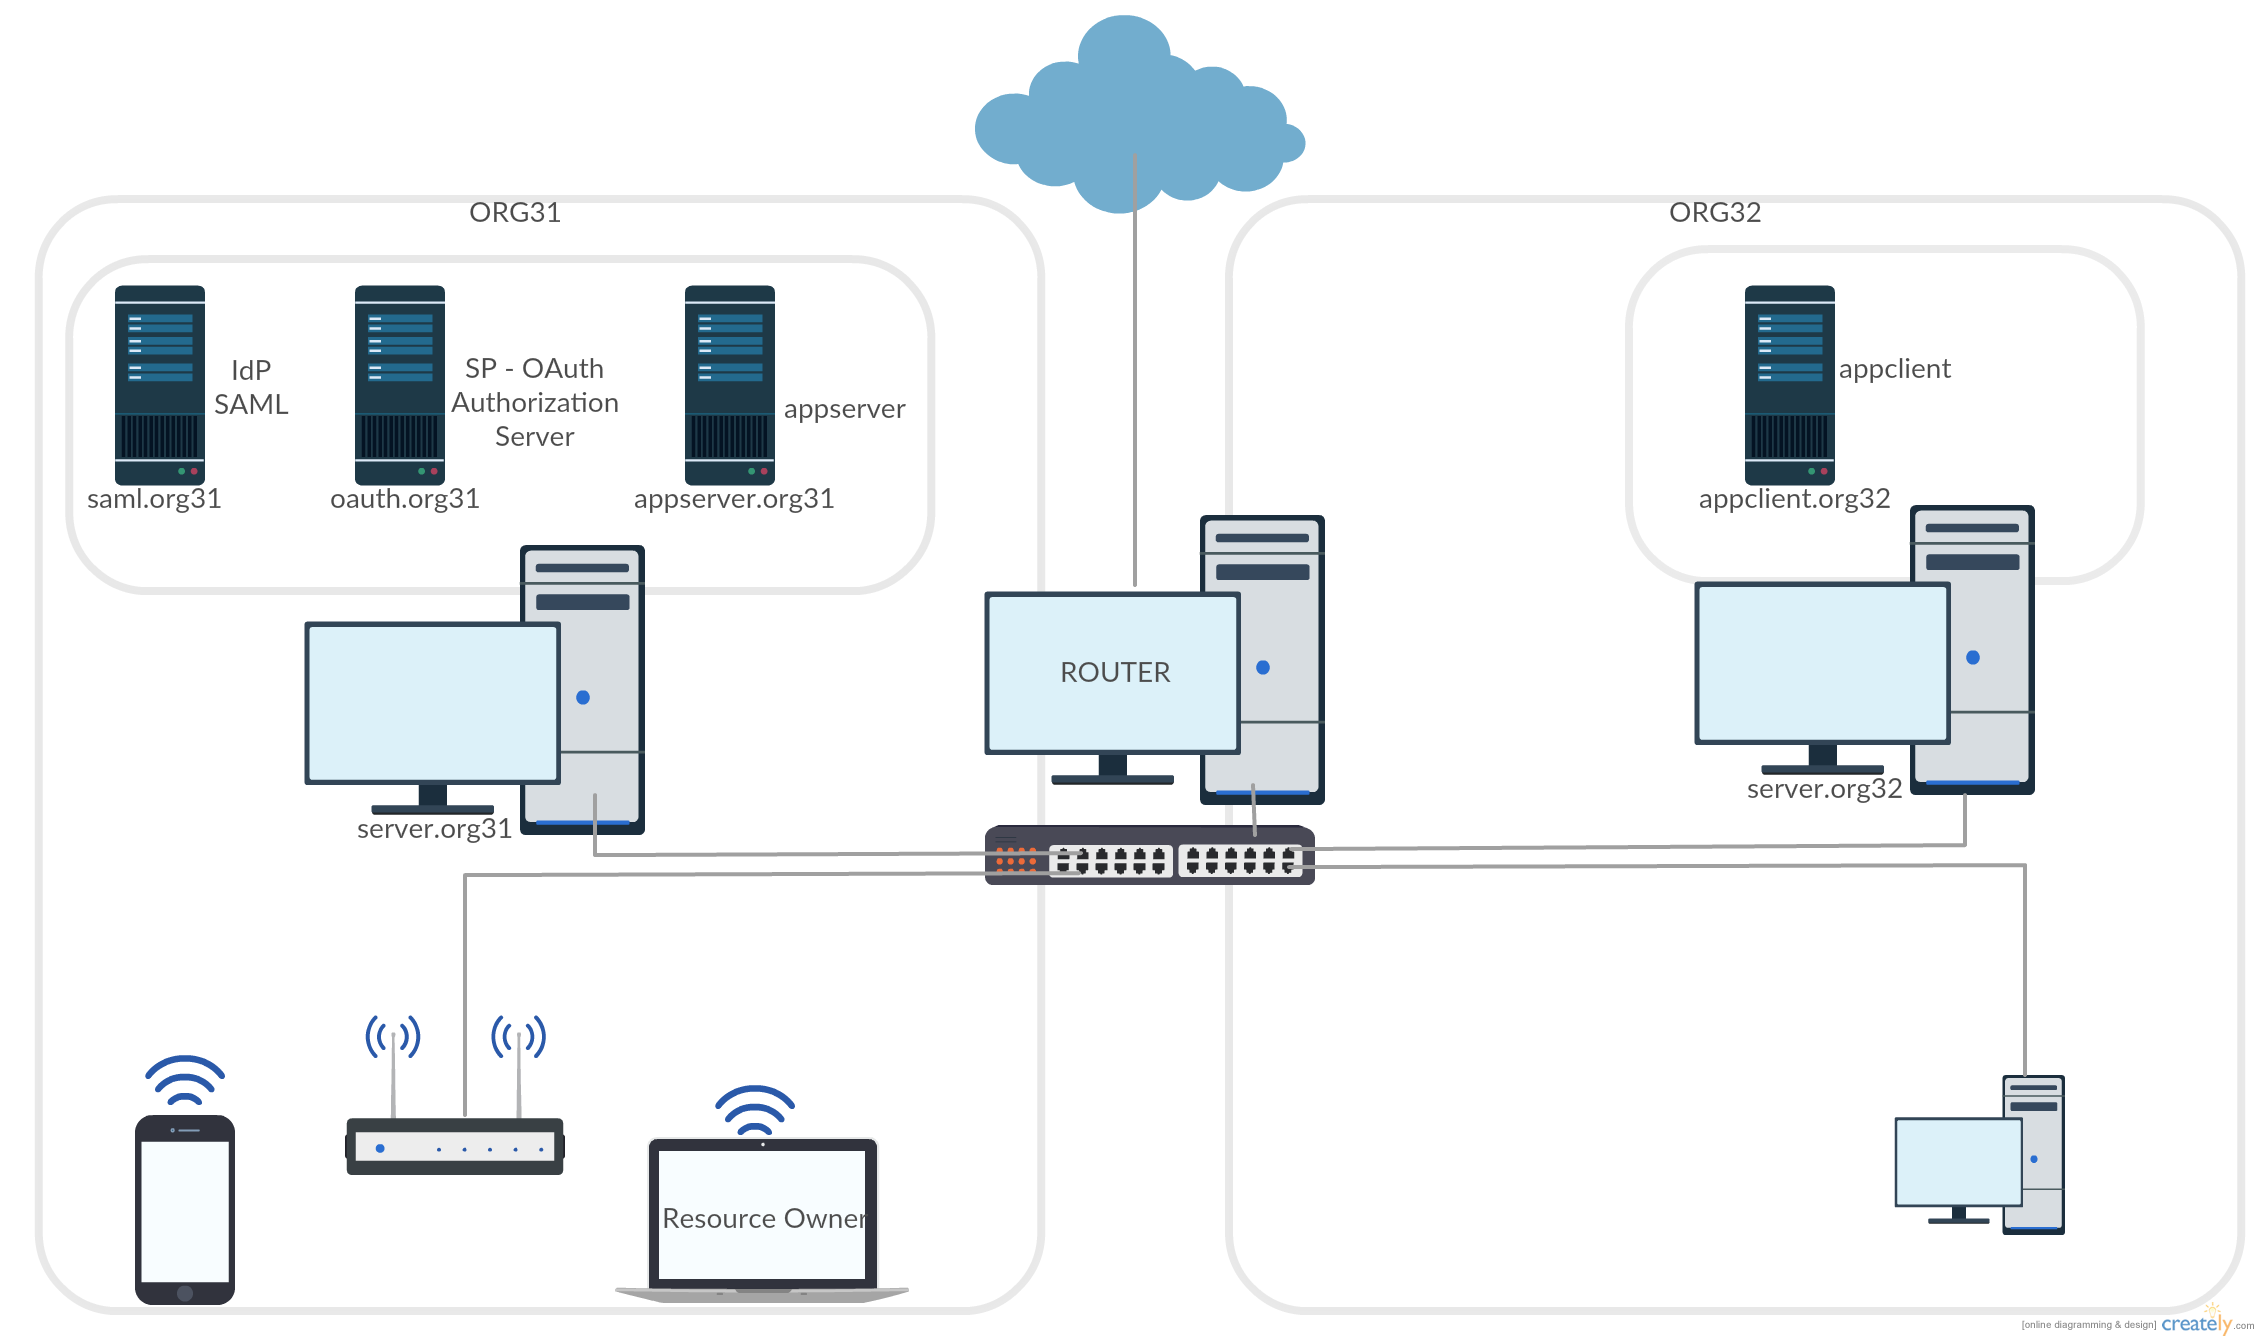
\includegraphics[width=1\linewidth]{images/samloauth/escenario.png}

	\textit{Escenario LEGO de gestión de identidad}
\end{center}

Se nos pide desarrollar un escenario donde el \textit{Resource Owner}, el usuario por medio de su explorador web, se conecta a \textit{appclient.org32},
donde quiere iniciar sesión. Al pinchar en \textit{Login} la web \textit{appclient} le redirige al servidor de \textbf{autorización}, donde pedirá poder acceder
a los datos del usuario para iniciar sesión. Esto se realizará por OAuth con la máquina \textit{oauth.org31}, estando aquí el principal cambio con respecto
a la arquitectura propuesta, que comentaremos por qué más adelante. En este punto \textit{oauth.org31} aún no sabe de qué usuario se trata, por eso necesita que
iniciemos sesión, pero como \textit{oauth.org31} no maneja los usuarios y credenciales, actúa como un \textit{SP} usando SAML con el IdP en la máquina \textit{saml.org31},
la cual sí tiene configurados los usuarios y contraseñas. Una vez nos \textbf{autenticamos} en \textit{saml.org31}, como \textit{Resource Owner} damos permiso en
\textit{oauth.org31} para dar los datos de inicio de sesión a \textit{appclient.org32}.


\hfill

Hemos cambiado \textit{oauth} de la Organización 32 a la Organización 31 debido a las complicaciones de separar la implementación del proyecto de Phillip Shipley en varias máquinas. Consideramos que la estructura actual sigue representando una situación de organizaciones realista. Poniendo de ejemplo Google y Doodle,
Doodle sería \textit{appclient} en la Organización 32, y Google sería \textit{oauth} como el servidor de autorización, el que muestra qué cosas compartirás con Doodle, como tu nombre y correo,
también será \textit{saml}, el IdP con el que iniciarás sesión, y puede añadir características extra como el \textit{second factor of authentication}, y también el \textit{appserver} por ejemplo
con la lista de contactos u otro elemento del que hayas dado permisos en la autorización de \textit{oauth}.

Como \textit{saml.org31} y \textit{oauth.org31} pertenecerían ambos a Google, pueden estar en la misma máquina.

\hfill

De querer separar el SP y el IdP en 2 máquinas partiendo del proyecto de Shipley, el procedimiento sería, para la máquina del IdP, seguir los pasos de instalación referentes al servicio \textit{saml}, para la máquina del SP, seguir los pasos de instalación referentes a los servicios \textit{php-oauth} y \textit{saml}, y ahora editar en los directorios \textit{simplesamlphp/} instalados, los ficheros \textit{config/authsources.php}, \textit{metadata/saml20-idp-remote.php}, \textit{metadata/saml20-idp-hosted.php} y \textit{metadata/saml20-sp-remote.php}, eliminando de la máquina SP lo referente a la configuración del IdP, y de la máquina del IdP lo referente a la configuración del SP, donde podemos ayudarnos de las diapositivas de la práctica 2.

\hfill

Repetimos que preferimos no hacerlo por falta de tiempo y porque hemos encontrado otras dificultades que no se podían dejar pasar en el diseño de un escenario realista.

\subsection{Scripts de instalación}

Para automatizar la configuración del escenario en cualquier máquina, hemos escrito una serie de scripts que no necesitan de interacción manual una
vez se inicia la instalación (excepto algún \textit{Enter} ocasional). Utilizamos la herramienta \textit{make} para facilitar aún más
el despliegue. La organización de los scripts corresponde a una jerarquía de directorios como la siguiente:

\hfil

\begin{BVerbatim}
ROUTER
	Makefile
	network
	test

ORG1
	SERVER
		Makefile
		network
		test
		ESCENARIO
			install.sh
			php-oauth-saml-demo-master
				appserver
				php-oauth
				simplesamlphp
				vagrant

ORG2
	SERVER
		Makefile
		network
		test
		ESCENARIO
			install.sh
			php-oauth-saml-demo-master
				appclient
				vagrant
\end{BVerbatim}

\hfill


Donde ESCENARIO sirve como carpeta contenedora de los scripts específicos de esta práctica, mientras que otros ficheros como \textit{network} nos
permiten configurar LEGO automáticamente, configurando la red, el forwarding, la resolución de DNS o fichero \textit{hosts}, etc.

%También usamos otros directorios, como SAML para la práctica 2, u OAUTH para la 3, de donde reutilizamos parte de los scripts para ESCENARIO.


\hfill

En la práctica, para ejecutarlos, basta con irse al directorio correspondiente, por ejemplo, para configurar la Organización 31, navegamos a ORG1/SERVER/, y desde ahí
ejecutamos la orden:

\begin{verbatim}
sudo make [network] [escenario] [saml] [test] [...]
\end{verbatim}

Si no ponemos argumentos, por defecto aplicaría la configuración de la red y test. De querer instalar la práctica 2, deberíamos indicar \textit{make saml}, y, para el escenario a entregar, \textit{make escenario}.

\hfill

Es importante notar que la configuración de la red (\textit{make network}) no sólo configura las IP de cada máquina, así como el \textit{forwarding} de la que haga de Router, sino que además configura el DNS de Google para navegar por internet, y en el fichero \textit{/etc/hosts} añade las entradas de \textit{server.org31}, \textit{server.org32}, \textit{oauth.org31}, \textit{appclient.org32}, etc., que se pueden ver en la imagen del escenario al inicio de esta sección. Esto último es de gran importancia porque así pasamos de usar los nombres \textit{*.local} del escenario de la práctica 3, a direcciones cualquiera que podrían estar en la jerarquía DNS, y al forzarnos a cambiarlos, nos daremos cuenta de cómo se podría mejorar este escenario de prácticas.


\subsection{Configuración de la Organización 31: appserver, php-oauth y simplesamlphp}



En el script de instalación en  \textit{ORG1/SERVER/ESCENARIO/} automatizamos la instalación de \textit{apahce2}, \textit{php}, la activación de \textbf{HTTPS}, y la copia de los ficheros de configuración de cada servicio.

\hfill

Los servicios web se configuran al modificar el fichero \textit{vagrant/vhost-local.conf}, eliminando la entrada de \textit{appclient}, cambiando los \textit{.local} por \textit{.org31} y duplicándolo en \textit{vagrant/vhost-secure.conf}, donde añadimos la configuración para \textbf{HTTPS}. Los certificados emitidos para \textit{appserver.org31}, \textit{oauth.org31} y \textit{saml.org31} están en el directorio \textit{CACERT/} y se copiarán en \textit{/etc/apache2/cert} en la instalación. Son autofirmados, pero al menos van emitidos a los nuevos nombres de dominio de cada servicio.

\hfill

En la configuración de \textit{appserver}, \textit{php-oauth} y \textit{simplesamlphp} hemos buscado en todos los ficheros de sus directorios cualquier referencia a \textit{appserver.local}, \textit{appclient.local}, \textit{php-oauth.local} y \textit{simplesamlphp.local}, para cambiarlos por \textit{appserver.org31}, \textit{appclient.org32}, \textit{php-oauth.org31} y \textit{simplesamlphp.org32}, o cualquier otro nombre de dominio que les hubiéramos asignado para poder acceder desde fuera de la máquina donde están instalados.

\hfill

Sin embargo, esto no fue suficiente, porque en las pruebas durante el desarrollo del script, una vez autorizábamos en \textit{oauth.org31} el uso de nuestros datos para \textit{appclient.org32}, nos redireccionaba a \textit{appclient.local}, y buscando incluso en los ficheros ya configurados por el \textit{composer.phar} y en toda la documentación que había disponible, no salían más referencias a \textit{appclient.local}.

El problema radicaba en el fichero de base de datos de sqlite en \textit{php-oauth/data/oauth2.sqlite}, donde el binario, usando un explorador de base de datos, vimos que en la tabla \textit{Client}, tenía 3 entradas para la configuración de \textit{oauth}, donde había referencias a las direcciones \textit{.local}. 

Una vez modificamos la base de datos con las nuevas direcciones, el escenario funcionó correctamente.

\hfill

En cuanto a \textbf{HTTPS}, hemos añadido su configuración y si accedemos a cada página con \textit{https://...}, aparte del aviso de que es un certificado autofirmado, todo funciona perfectamente. El problema es, en cada fichero que hemos modificado para eliminar los \textit{.local}, algunas líneas eran parte de las órdenes \textit{redirect}, y llevan explícitamente \textit{http://}, de modo que para que el escenario de pruebas funcione con HTTPS automáticamente, deberíamos localizar los \textit{redirect} y modificarlos por \textit{https://} y volver a aplicar el script de instalación y reiniciar el servicio.

No lo hacemos porque entonces no podríamos tomar las muestras de las trazas con wireshark, pues ahora se usaría forzadamente HTTPS.


\hfill

Ahora, en cuanto a la configuración de SAML para \textit{saml.org31} como IdP y para \textit{oauth.org31} como SP, debemos modificar algunos ficheros más, varios ya modificados al cambiar los \textit{.local}.

En \textit{simplesamlphp/metadata/} modificamos:
\begin{itemize}
	\item
	\textit{saml20-idp-hosted.php} para indicar que los nuevos ficheros del certificado de firma son \textit{saml.org31.pem} y \textit{saml.org31.crt}, que son los mismos que usa HTTPS para \textit{saml.org31}, autofirmados, pero que usará SAML para firmar los mensajes, no para cifrar la comunicación.
	
	\item
	\textit{saml20-idp-remote.php} para modificar los datos criptográficos que tiene el SP sobre el IdP (pues le hemos dado un nuevo certificado al IdP). Lo hacemos copiando y pegando el \textit{\$metadata} que da la web de \textit{simplesamlphp}, como hicimos en la práctica 2.
\end{itemize}

En \textit{simplesamlphp/config/authsources.php} añadimos la configuración de \textbf{Facebook}, la única aplicación externa de las que ofrece \textit{simplesamlphp} que no tiene una configuración obsoleta, es decir, que al añadir su \textit{api\_key} y su \textit{secret}, consigue conectarse a Facebook e identificarse como la app que hemos generado previamente en el área de desarrolladores. También probamos con Twitter, que al probarlo se queda una web en blanco, pues la URL de llamada de vuelta no parecía poder configurarse correctamente. Google hace tiempo que ya no soporta Open-ID, por lo que tampoco podíamos configurarlo. Windows Live tampoco existe ya, el servicio pasó a Onedrive y \textit{simplesamlphp} tiene todas la URL mal configuradas. Y Yubikey tampoco funcionaba al configurar su \textit{id} y \textit{key}, pero ignoramos qué fallo tendrá \textit{simplesamlphp} para no funcionar.

\hfill

Para terminar de configurar \textbf{Facebook}, debemos crear el fichero \textit{simplesamlphp/modules/authfacebook/enable}, que puede estar vacío, para que el módulo se active.

\hfill

Si nos conectamos a \textit{saml.org31}, en la pestaña \textit{Autenticación}, en el enlace \textit{Probar las fuentes para la autentificación ya configuradas}, podemos comprobar que funciona la identificación por Facebook, y que una vez autorizamos a usar nuestros datos, Facebook funciona como IdP y servidor de autorización, y nuestro test como \textit{appclient}.










\subsection{Configuración de la Organización 32: appclient}


Si nos vamos al directorio \textit{ORG2/SERVER/ESCENARIO/} nos encontramos el script de instalación que automatiza el proceso. Nos instala \textit{apache2}, activa el cifrado para usar \textbf{HTTPS}, instala las dependencias de \textit{php5}, y copia los ficheros de \textit{appclient}, modificados como ahora indicaremos, de los \textit{virtual hosts} de Apache2 y los certificados.

Configura el directorio de \textit{appclient} con php y reinicia el servicio de Apache2.

Todo muy sencillo y sin intervención humana.


\hfill


Ahora bien, hemos tenido que modificar algunos ficheros de como estaban en el repositorio original. En los ficheros \textit{protected/config/main.php} y \textit{protected/controllers/AuthController.php} tenemos que modificar todas las referencias de \textit{oauth.local}, \textit{appserver.local} y \textit{appclient.local} por las direcciones \textit{oauth.org31}, \textit{appserver.org31} y \textit{appclient.org32}, o el nombre real del DNS que tuviera cada máquina.

Por supuesto, hemos cambiado también el fichero \textit{vagrant/vhost-local.conf} para borrar los \textit{virtual host} de \textit{oauth}, \textit{saml} y \textit{appserver}, y cambiar \textit{appclient.local} por \textit{appclient.org32}.

\hfill

El certificado generado para \textit{CN=appclient.org31} se encuentra en el directorio \textit{CACERT/} del proyecto, y es el que se copia en \textit{/etc/apache2/cert} para que la configuración de los \textit{virtual host} con SSLEngine los utilice en HTTPS.



\hfill


Con estos cambios y el script la máquina \textit{server.org32} sirve la web \textit{appclient.org32} correctamente a cualquier otra máquina de la red. \textbf{De haber dejado \textit{appclient.local} fijo}, sin cambiarlo por \textit{appclient.org32}, o por cualquier otro nombre resoluble por DNS, \textbf{el escenario sólo funcionaría si el cliente, \textit{Resource Owner} se conectase desde la misma máquina donde está instalado \textit{appclient}}, y consideramos ese caso mucho menos realista que tener los servicios \textit{saml}, \textit{php-oauth} y \textit{appserver} en la misma máquina.



\section{Análisis de trazas}

Normalmente capturaríamos las trazas con Wireshark, y las interpretaríamos. Sin embargo, existe una herramienta llamada SAML Tracer (es un complemento de Firefox) que, si se utiliza mientras hacemos el login Single Sign On, muestra los intercambios y permite extraer el intercambio SAML. Con este intercambio podemos ahorrar tiempo ya que SAML viaja a través de HTTP, y no tenemos intención de analizar las trazas HTTP.

Si entramos en appclient.org32, hacemos login (que nos redirige a saml.org31, el IdP), y nos autenticamos como \textbf{user1}, se realizan dos intercambios SAML. El primero, es un intercambio de appclient de org32 para saml de org31, indicando que alguien quiere autenticarse, y el segundo, después de haber hecho login en saml.org31, va desde saml en org31 para appclient en org32, indicando información del usuario.

La traza completa con ambos intercambios es:

%TODO: incluir aquí el fichero anexos/traza.txt

De esta traza destaco los siguientes apartados XML:

\begin{itemize}
	\item <samlp:AuthnRequest ...> indica una petición de autenticación, con ID="\_49881caa8878bdd61c79da8c16d70a77d493e2e30e". Este id es importante, es al que tendrá que responder el IdP.
	\item Dentro del samlp:AuthnRequest el Destination="http://saml.org31/saml2/idp/SSOService.php" indica a donde tiene que dirigirse el cliente a completar la petición.
	\item Dentro también del samlp:AuthnRequest se encuentra AssertionConsumerServiceURL="http://oauth.org31/module.php/saml/sp/saml2-acs.php/oauth-sp", a donde habrá que volver una vez obtenida la respuesta.
	\item <samlp:Response ...> es la etiqueta XML para la respuesta a la petición. Se sabe que es respuesta a la petición anterior porque el campo InResponseTo="\_49881caa8878bdd61c79da8c16d70a77d493e2e30e" coincide exactamente con el ID de la petición.
	\item En ds:Signature y en las etiquetas hijas, está la firma de la respuesta. La respuesta la firma digitalmente el IdP para que los servicios puedan fiarse de la información que el cliente está transportando. Contiene información de como se firma el mensaje, así cómo el certificado del IdP.
	\item El StatusCode [...] Success indica que el intento de login fue correcto. 
	%TODO: hay elementos que no sé para que sirven después del status.
	\item Al final de la traza, hay unos atributos que indican el nombre de usuario, los grupos a los que pertenece (person, member) y sus roles (applications, administration).
\end{itemize}

\section{Conclusiones}

El escenario a configurar en el proyecto LEGO creemos que es bastante realista y complejo, sin pasarse en cantidad de servicios a configurar, como para entender bien la diferencia entre SAML para \textbf{autenticación} y de OAuth para \textbf{autorización}, y de cómo pueden trabajar conjuntamente, siendo cómodos de usar para el usuario final, y transparentes en cómo está realmente desplegado, permitiendo, en un escenario real, complicarlo lo que se quiera, de cara a añadir prestaciones y seguridad.

\hfill

Sin embargo, siendo el escenario muy correcto, no creemos que el punto de partida del proyecto de Phillip Shipley sea el idóneo. Sí lo es para la práctica 3, donde con un script de \textit{vagrant} se tiene el escenario de una máquina totalmente desplegado. Pero en la parte de llevarlo al mundo real, no tiene tan bien definidos en de los ficheros, qué configuración pertenece a qué servicio, y es muy difícil descubrir que hay referencias a los nombres \textit{*.local} incluso en ficheros binarios de bases de datos.

\hfill

De cara al siguiente curso que deba desplegar esta práctica, recomendaríamos que se modificara el proyecto de Shipley. Por medio de un fichero global de configuración, se mapearían las direcciones de cada servicio con su nombre de dominio final, por ejemplo con el formato:

\begin{verbatim}
$appclient = cliente.um.es
$appserver = servidor.com
$oauth = authZ.edu
$saml = idp.org
\end{verbatim} 

Y con un script (bash, python, ...) que lo leyera y modificara cada fichero que hemos mencionado en esta memoria (donde hemos cambiado un \textit{.local} por un \textit{.org3N}).

Un modo sería aprovechar que son ficheros php, cambiar las referencias a \textit{appclient.local}, etc., por variables, y que el script modifique lea los nombres de dominio y modifique las variables.

Todavía quedaría el tema de la base de datos de \textit{php-oauth}, la cual modificaríamos por sólo la definición, y que en la instalación, al igual que hacemos un \textit{php composer.phar install}, añadir un script que rellene la base de datos.


\hfill


Al final para el alumno quedaría un proyecto tan cómodo como el de Shipley, pero donde por un fichero global puede separarlo en varias máquinas, por medio de una mejor documentación del apartado de \textit{simplesamlphp}, puede separar \textit{oauth} como SP de \textit{saml} como IdP. Quedaría entonces un escenario más realista, donde el alumno aún debe pelearse con OAuth y SAML, identificar sus \textit{roles}, pero no se pelea con partes del proyecto que no tienen relevancia real en la parte de autenticación y autorización.



\end{document}
